\chapter{Aplicaciones continuas}%
\label{cha:aplicaciones_continuas}

\section{Continuidad}%
\label{sec:continuidad}
Recordemos el famoso $\varepsilon-\delta$ en $\left( \mathbb{R}^n, \mathcal{T}_u \right)$, sea $x_0 \in X$ y $f : X \rightarrow Y$, será continua si y solamente si: 
\begin{gather*}        
\forall \varepsilon > 0, \exists \delta > 0: 
\begin{cases}
    \lVert x - x_0 \rVert < \delta \Rightarrow \lVert f\left( x \right) - f\left( x_0 \right) \rVert < \varepsilon \\
    x \in B\left( x_0, \delta \right) \Rightarrow f\left( x \right) \in B\left( f\left( x_0 \right), \varepsilon \right) \\
    f\left( B\left( x_0, \delta \right) \right) \subset B\left( f\left( x_0 \right), \varepsilon \right) 
\end{cases}
.\end{gather*}
Todas estas equivalencias se pueden traducir a:
\[
\boxed{\forall B\left( f\left( x_0 \right), \varepsilon \right),\ \exists B\left( x_0, \delta \right) \subset f^{-1}\left( B\left( f\left( x_0 \right), \varepsilon \right) \right)} 
\]
que es similar a la definición que nos interesa.

\begin{defi}[Continuidad]
Sea $f: X \rightarrow Y$ una función entre espacios topológicos, decimos que es \textbf{continua en $x_0$ $\in X$} si y sólo si:
\[
\forall V^{f\left( x_0 \right)} :  f^{-1}\left( V^{f\left( x_0 \right)} \right) = V^{x_0} 
\]
es decir, la preimagen de cualquier entorno de $f(x_0)$ es entorno de $x_0$.
\end{defi}

\begin{prop}[Composición de continuidades]
Sean $f:X \rightarrow Y$ y $g: Y \rightarrow Z$ funciones continuas en $x_0\in X$ e $y_0\in Y$ tales que $f(x_0) = y_0$, entonces la composición $h = g \circ f$ es una función continua en $x_0$.
\end{prop}
\begin{demo}
Escojamos un entorno $V^{h\left( x_0 \right)}$ de la imagen por $h$ de $x_0$, entonces
\[
h^{-1} V^{h\left( x_0 \right)} = f^{-1}g^{-1}V^{g\left( y_0 \right)} = f^{-1} V^{y_0} = V^{x_0}
\]
\end{demo}

\begin{ej}
\begin{enumerate}
    \item Sea $f: X_{\text{discreta}} \rightarrow Y$, entonces es continua sean cuales sean los conjuntos de partida y de llegada, pues todo es abierto y, en consecuencia, todo es entorno en $\mathcal{T}_{\text{disc}}$.
    \item Sea $f: X \rightarrow Y_{\text{trivial}}$, entonces es continua sean cuales sean los conjuntos de partida y de llegada, pues como $Y$ es el único abierto, entonces es el único entorno $V^{f\left( x \right)}$ para cualquier $f(x)$ y $f^{-1}V^{f\left( x \right)} = f^{-1}Y = X$, que es abierto.
    \item Si una función $f: X \rightarrow Y_{\text{discreta}}$ es continua, entonces $f$ es localmente constante, pues como en la trivial los puntos son abiertos, entonces el punto $\{f\left( x_0 \right)\}$ es entorno $V^{f\left( x_0 \right)}$ de sí mismo. Por tanto, por la continuidad de $f$, $f^{-1}f\left( x_0 \right) = V^{x_0}$, luego $f \equiv f\left( x_0 \right)$ en ese entorno $V^{x_0}$.
    \item Si una función $f: X \rightarrow Y$ es localmente constante, entonces es continua, puesto que si es localmente constante para cualquier $x_0 \in X$ existe un entorno $U^{x_0} : f\mid_{U^{x_0}} \equiv f\left( x_0 \right)$. De este modo, cualquier entorno $V^{f\left( x_0 \right)}$ de la imagen $f(x_0)$ cumple que $f^{-1}V^{f\left( x_0 \right)} \supset U^{x_0}$ y llamando $V^{x_0} = f^{-1} V^{f\left( x_0 \right)}$ entonces vemos que es entorno de $x_0$.
\end{enumerate}
\end{ej}

\begin{prop}[Caracterización de Continuidad]
Sea $f:X\rightarrow Y$ una función entre espacios topológicos, entonces son equivalentes:
\begin{enumerate}
    \item $f$ es continua.
    \item $\forall U \stackrel{\text{ab.}}{\subset} Y : f^{-1}\left( U \right) \stackrel{\text{ab.}}{\subset} X$.
    \item $\forall F \stackrel{\text{cerr.}}{\subset} Y : f^{-1}\left( F \right) \stackrel{\text{cerr.}}{\subset} X$.
    \item $\forall A \subset Y : f^{-1}\left( \mathring{A} \right) \subset \inter\left( f^{-1}\left( A \right) \right)$.
    \item $\forall A \subset X : f\left( \overline{A} \right) \subset \overline{f\left( A \right)}$.
\end{enumerate}
\end{prop}
\begin{demo}
\begin{itemize}
    \item $1 \Rightarrow 2)$
    
    Escojamos un abierto cualquiera $W \stackrel{\text{ab.}}{\subset} Y$. Por ser abierto, es entorno de todos sus puntos y, en particular, es entorno de las imágenes que puedan caer dentro de dicho abierto, es decir, $\forall x \in f^{-1} (W) : W = V^{f(x)}$. Por continuidad, las preimágenes de entornos de las imágenes son entornos de las preimágenes, luego $\forall x \in f^{-1} W : f^{-1}W = V^x$ y como es entorno de todos sus puntos, entonces $f^{-1} W \stackrel{\text{ab.}}{\subset} X$.
    \item $2 \Rightarrow 3)$
    
    Como lo que sabemos es que las preimágenes de abiertos son abiertas y los cerrados se definen en términos de abiertos, no nos queda otra estrategia que intentar demostrarlo pasando los cerrados a sus complementarios: los abiertos.
    
    Escojamos un cerrado cualquiera $C \stackrel{\text{cerr.}}{\subset} Y$ de modo que conocemos que $Y \setminus C \stackrel{\text{ab.}}{\subset} Y$. Como conocemos el resultado para abiertos, podemos decir que $f^{-1}\left( Y\setminus C \right) \stackrel{\text{ab.}}{\subset} X$ y, conjuntistamente, $X \setminus f^{-1}C = f^{-1}\left( Y\setminus C \right)$, luego directamente tenemos que $f^{-1}C \stackrel{\text{cerr.}}{\subset} X$. 
    \item $3 \Rightarrow 5)$

    \[
        \overline{f\left( A \right)} \stackrel{\text{cerr.}}{\subset} Y \xRightarrow{3)} \underbrace{f^{-1}\overline{f\left( A \right)}}_{\subset f^{-1}f\left( A \right) \supset A} \subset X \Rightarrow \overline{A} \subset f^{-1}\overline{f\left( A \right)} \Rightarrow f\left( \overline{A} \right) \subset \overline{f\left( A \right)} 
    \]
    \item $5 \Rightarrow 4)$
    \begin{gather*}
        Y \setminus \mathring{A}\Rightarrow \overline{Y\setminus A} \supset \overline{f\left( X \setminus f^{-1}A \right)} \stackrel{5)}{\supset} f\left( \overline{X \setminus f^{-1}\left( A \right)} \right) = f\left( X \setminus \inter\left( f^{-1}A \right) \right) \Rightarrow\\
        X \setminus \inter\left( f^{-1}A \right) \subset f^{-1}\left( Y\setminus \mathring{A} \right) = X \setminus f^{-1}\left( \mathring{A} \right)\Rightarrow f^{-1}\left( \mathring{A} \right) \subset \inter\left( f^{-1}A \right) 
    .\end{gather*}

    \item $4 \Rightarrow 1)$
    \begin{gather*}
        V^{f\left( x \right)} \Rightarrow f\left( x \right) \in \inter\left( V^{f\left( x \right)} \right) \Rightarrow x \in f^{-1}\left( \inter\left( V^{f\left( x \right)} \right) \right) \subset \inter\left( f^{-1}V^{f\left( x \right)} \right) \Rightarrow \\
        f^{-1}V^{f\left( x \right) } \text{ entorno de } x.
    \end{gather*}
\end{itemize}
\end{demo}

\begin{obs}
\begin{enumerate}
    \item Los cuatros primeros enunciados tratan sobre ``imágenes inversas''. Por ejemplo, la segunda dice que $f^{-1}\mathcal{T}_Y \subset \mathcal{T}_X$.
    \item Pensando que un punto adherente es un ``punto límite'', $5$ nos dice que ``la imagen del límite es el límite de la imagen''.
    \item $id: \left( X, \mathcal{T}_1 \right) \rightarrow \left( X, \mathcal{T}_2 \right)$ es continua $\Leftrightarrow \mathcal{T}_2 \subset \mathcal{T}_1$ (por 1). 
\end{enumerate}
Y no mencionamos todos los ejemplos conocidos en espacios afines $\mathbb{R}^n$ con $\mathcal{T}_u$.
\end{obs}


\section{Continuidad y subespacios}%
\label{sec:continuidad_y_subespacios}
\begin{prop}
Sea $f: X \rightarrow Y$ una función continua y $Z \subset X$ un subespacio topológico, entonces la restricción $f|_Z : Z \rightarrow Y$ también es continua.
\end{prop}
\begin{demo}
Aplicando la caracterización de continuidad a través de las preimágenes de abiertos, tenemos que:
\[
\forall A \stackrel{ab}{\subset} Y : \left( f|_Z \right)^{-1} \left( A \right) = Z \cap f^{-1} A \stackrel{ab}{\subset} Z
\]
donde este último conjunto es abierto por ser un abierto ambiente cortado con el subespacio (que es como son los abiertos de la topología relativa).
\end{demo}

%TODO: Diagramas composición
\begin{obs}
\begin{enumerate}
    \item $Z \stackrel{j}{\subset} X$ es continua.
    \begin{demo}
        \begin{itemize}
            \item $z \in Z: \forall V^{j\left( z \right)} : \underbrace{j^{-1}\left( V^{j\left( z \right) } \right)}_{= V^{j\left( z \right)} \cap Z}$ entorno de $z$ en $Z$.
            \item $\forall U \stackrel{\text{ab.}}{\subset } X: \underbrace{j^{-1}\left( U \right)}_{U \cap Z} \stackrel{\text{ab.}}{\subset} Z$
        \end{itemize}
    \end{demo}

    \item $Z \stackrel{j}{\subset} X \xrightarrow{f} Y$. Si $f$ es cont. $\Rightarrow f|_Z$ continua. (No a la inversa).
    \begin{demo}
    Como $f|_Z = f \circ j$ y ambas son continuas, por composición, $f|_Z$ es continua.
    \end{demo}

    \item La continuidad es \underline{local}. 

    Si $f|_{E^x}$ continua en $x \Rightarrow f$ continua en $x$.
    \begin{demo}
        $\forall V^{f\left( x \right)} \Rightarrow \left( f|_{E} \right)^{-1} \left( V^{f\left( x \right)} \right) = W^x$ entorno de $x$ en $E^x$.

        Como $W^x \stackrel{\text{ent.}}{\subset} E^x \stackrel{\text{ent.}}{\subset} X \Rightarrow W^x \stackrel{\text{ent.}}{\subset}X$ (entorno en entorno es entorno). Porque, 
        \[
        \begin{rcases}
            x \in W^x: \exists G \stackrel{\text{ab.}}{\subset} W^x \subset E^x: G = A \cap E^x \subset X\\ 
            x \in E^x: \exists B \stackrel{\text{ab.}}{\subset} E^x \subset X 
        \end{rcases} \Rightarrow x \in \underbrace{A \cap B}_{\stackrel[\text{ab.}]{}{\subset} X} \subset \underbrace{A \cap E^x}_{= G}  \subset W^x
        \]
    \end{demo}

    \item Si $f|_{U \stackrel{\text{ab.}}{\subset} X}$ es continua $\Rightarrow f$ continua $\forall x \in U$.

    \item $x$ es aislado $\Rightarrow f$ continua en $x$. 
    \begin{demo}
        $x$ aislado $\Leftrightarrow V^x = \{x\}$ es abierto de $X$. $f|_{V^x} : \{x\} \rightarrow Y$.
    \end{demo}

    \item $f: X \rightarrow Y \supset Z$ tal que $f\left( X \right) \subset Z \subset Y$ (si no es así puede estar mal definido).

    Entonces, $f$ a $Y$ es continua $\Leftrightarrow f$ a $Z$ es continua.
    \begin{demo}
        \begin{itemize}
            \item $f$ cont. en $Z \xRightarrow{j \circ f} f$ cont. en $Y$. %TODO: Seguro?
            \item $f$ cont. en $Y \xRightarrow{?} f$ cont. en $Z$. 

            Sea $U_z$ ab. en $Z$. Este será $U_y \cap Z = U_z$ que cumple, $f_z^{-1}\left( U_y \cap Z \right) \stackrel{f\left( X \right) \subset Z}{=}  f_y^{-1}\left( U_y \right)$ que es abierto en $X$ (por ser $f_y$ continua).
        \end{itemize}
    \end{demo}
\end{enumerate}
\end{obs}

\begin{prop}[Criterios de continuidad por recubrimientos]
Sea $f: X \rightarrow Y$ una función entre espacios topológicos, si se da alguna de las siguientes condiciones: 
\begin{align*}
\begin{cases}
X = \bigcup_{i \in  I} U_i \mbox{ donde } U_i \stackrel{\text{ab.}}{\subset} X \\
\forall f|_{U_i} : U_i \rightarrow Y \mbox{ cont.}
\end{cases}
& &
\begin{cases}
X = \bigcup_{i =0}^n F_i \mbox{ donde } F_i \stackrel{\text{cerr.}}{\subset} X \\
\forall f|_{F_i} : F_i \rightarrow Y \mbox{ cont.}
\end{cases}
\end{align*}
entonces la función $f$ del inicio es continua.
\end{prop}
\begin{demo}
	\begin{itemize}
	\item Escojamos un abierto cualquiera $W \stackrel{\text{ab.}}{\subset} Y$ y veamos si su preimagen $f^{-1}W$ es un abierto en $X$.

    En primer lugar, por ser $X = \bigcup_{i \in  I} U_i$ podemos escribir que $f^{-1}W = X\cap f^{-1}W = \bigcup_{i \in  I} U_i \cap f^{-1} W = \bigcup_{i \in  I} \left( U_i \cap f^{-1} W\right) = \bigcup_{i \in  I} \left( f|_{U_i} \right)^{-1} W$. Como $\left( f|_{U_i} \right)^{-1}W \stackrel[\text{(cont.)}]{\text{ab.}}{\subset} U_i \stackrel{\text{ab.}}{\subset} X$, entonces $\left( f|_{U_i} \right)^{-1} W \stackrel{\text{ab.}}{\subset} X$ y de esta manera podemos escribir $f^{-1}W$ como unión de abiertos $\bigcup_{i \in  I} \left( f|_{U_i} \right)^{-1} W$ de $X$, es decir, que $f^{-1}W \stackrel{\text{ab.}}{\subset} X$.
	
	\item Escojamos un cerrado cualquiera $C \stackrel{\text{cerr.}}{\subset} Y$ y veamos si su preimagen $f^{-1}C$ es cerrada en $X$.

    En primer lugar, por ser $X = \bigcup_{i=0}^n F_i$ podemos escribir que $f^{-1}C = X\cap f^{-1}C = \bigcup_{i = 0}^n F_i \cap f^{-1} C = \bigcup_{i = 0}^n \left( F_i \cap f^{-1} C\right) = \bigcup_{i = 0}^n \left( f|_{F_i} \right)^{-1} C$. Como $\left( f|_{F_i} \right)^{-1}C \stackrel[\text{(cont.)}]{\text{cerr.}}{\subset} F_i \stackrel{\text{cerr.}}{\subset} X$, entonces $\left( f|_{U_i} \right)^{-1} C \stackrel{\text{cerr.}}{\subset} X$ y de esta manera podemos escribir $f^{-1}C$ como unión finita de cerrados $\bigcup_{i = 0}^n \left( f|_{F_i} \right)^{-1} C$ de $X$, es decir, que $f^{-1}C \stackrel{\text{cerr.}}{\subset} X$.
    \end{itemize}
\end{demo}


\section{Homeomorfismos}%
\label{sec:homeomorfismos}
Recordemos las definiciones de continuidad que hemos visto:
\[
f \text{ continua} \Leftrightarrow f^{-1}\left( \text{abierto} \right) = \text{abierto} \Leftrightarrow f^{-1}\left( \text{cerrado} \right) = \text{cerrado} 
\]
Ahora veamos que ocurre al invertir la relación.
\begin{defi}[Aplicaciones abiertas y cerradas]
Sea $f: X \rightarrow Y$ una función entre espacios topológicos, decimos que es:
\begin{itemize}
\item \textbf{abierta} si y sólo si las imágenes de abiertos son abiertos.
\item \textbf{cerrada} si y sólo si las imágenes de cerrados son cerrados.
\end{itemize}
\end{defi}

\begin{obs}
La caracterización que dimos de la continuidad hacía referencia a las preimágenes de abiertos y cerrados, no a sus imágenes. De hecho, ni la continuidad implica que la aplicación sea abierta o cerrada, ni viceversa.
\end{obs}

\begin{ej}
En la siguiente tabla podemos ver distintos ejemplos de funciones que verifican algunas de las condiciones que hemos definido, pero no otras simultáneamente:
\begin{center}
\begin{tabular}{c|c|c|c}
Función & continua & abierta & cerrada \\
\hline
$Id: X_{\text{trivial}} \rightarrow X_{\text{discreta}}$ & \ding{55} & \checkmark & \checkmark \\
\hline
$Id: X_{\text{discreta}} \rightarrow X_{\text{trivial}}$ & \checkmark & \ding{55} & \ding{55} \\
\hline
$j: \left[ 0, 1 \right] \subset \mathbb{R}_{u}$ & \checkmark & \ding{55} & \checkmark \\
\hline
$j: \left( 0, 1 \right) \subset \mathbb{R}_u$ & \checkmark & \checkmark & \ding{55} \\
\hline
\end{tabular}
\end{center}
\end{ej}

\begin{prop}[Trivialidades esenciales]
Sea $f:X\rightarrow Y$ una función biyectiva, entonces las siguientes afirmaciones son equivalentes:
\begin{itemize}
    \item $f$ es abierta
    \item $f$ es cerrada
    \item $f^{-1}$ es continua.
\end{itemize}
\end{prop}
\begin{demo}
\begin{enumerate}
    \item $F_{\text{cerr}} \subset X \Rightarrow X\setminus F_{\text{ab}} \subset X \Rightarrow^{ f\text{ ab}} \underbrace{f\left( X\setminus F \right)}_{= Y\setminus f\left( F \right) \text{(biy.)}} \subset_{\text{ab}} X \Rightarrow f\left( F \right) \subset_{\text{cerr}} Y \Rightarrow f$ cerr.

    \item $F_{cerr} \subset X \Rightarrow^{f \text{cerr}} \underbrace{f\left( F \right)}_{= \left( f^{-1} \right)^{-1} \left( F \right) \text{(biy)}} \subset_{\text{cerr}} Y \Rightarrow f^{-1}$ cont.

    \item $U_{\text{ab}} \subset X \Rightarrow^{f^{-1} \text{cont}} \underbrace{\left( f^{-1} \right) ^{-1} \left( U \right) }_{f\left( U \right) \text{(biy.)}} \subset Y \Rightarrow f$ ab.
\end{enumerate}
\end{demo}

\begin{defi}[Homeomorfismo]
Sea $f: X \rightarrow Y$ una aplicación biyectiva, decimos que es un \textbf{homeomorfismo} si y sólo si $f$ y $f^{-1}$ son continuas, o equivalentemente si:
    \[
    \begin{cases}
        f \text{ biy.}\\
        \text{cont.}\\
        \text{ab.} 
    \end{cases} \Leftrightarrow \begin{cases}
        f \text{ biy.}\\
        \text{cont.}\\
        \text{cerr.}
    \end{cases} 
    \]
\end{defi}

%TODO: Arreglar mix
\begin{obs}
\begin{itemize}
    \item Cuando $f$ es homeomorfismo establecemos una biyección entre las topologías:
    \begin{align*}
        f: \mathcal{T}_X &\rightarrow \mathcal{T}_Y\\
        U &\mapsto f\left( U \right)\\
        f^{-1}\left( W \right) &\mapsfrom W 
    .\end{align*}

    %TODO: Tal vez, eliminar?
    \item Se conserva por rotación, por composición.
\end{itemize}
\end{obs}

\begin{defi}[Homeomorfismo Local]
Sea $f: X \rightarrow Y$ una función entre espacios topológicos, decimos que es un \textbf{homeomorfismo local en $x_0 \in X$} si y sólo si $f: V^{x_0} \rightarrow V^{f\left( x_0 \right)}$ restringida a algunos entornos de $x_0$ y $f\left( x_0 \right)$ es homeomorfismo.

Será \textbf{homeomorfismo local} si lo es en todo el dominio.
\end{defi}

\begin{obs}
Se pueden tomar $V^{x_0}, V^{f\left( x_0 \right)}$ entornos abiertos.
%TODO: Corregir
\begin{demo}
Si $V^a \subset X$ y $V^{f\left( a \right)} \subset Y$, tenemos: 
\[
    f: V^a \rightarrow V^{f\left( a \right)}
\]
Sabemos que $\exists U^a (\stackrel{\text{ab.}}{\subset} V^a) \mapsto f\left( U^a \right) (\stackrel{\text{ab.}}{\subset} V^{f\left( a \right)})$ al ser homeomorfismo. 

Además, como $f$ es abierto, local en $V^{f\left( a \right)}$ (homeomorfismo local), $f\left( U^a \right)$ es entorno de $f\left( a \right)$, pero no abierto (tal vez sí). 

Por tanto, tiene un abierto ($W^{f\left( a \right)} \subset f\left( U \right)$) que es imagen de un abierto, $G$, en $X \rightarrow f\left( G \right) = W^{f\left( a \right)} \stackrel{\text{ab.}}{\subset} Y$, con $G \stackrel{\text{ab.}}{\subset} X$.
\end{demo}
\end{obs}

\begin{prop}[Restricción de homeomorfismos]
Sea $f: X \rightarrow Y$, la restricción a $Z \subset X$ también es homeomorfismo: $f: Z \rightarrow f\left( Z \right)$.
\end{prop}
\begin{demo}
%TODO: No sé si está bien, me lo he inventado yo.
La restricción será biyectiva por serlo $f$ (y por estar restringida la llegada $Y$). Una biyección es homeomorfismo si son continuas ellas y su inversa, pero como ya vimos la restricción de una continua es continua, por lo tanto, la restricción de $f$ y $f^{-1}$ a $Z$ y $f\left( Z \right)$ son también continuas. Es decir, $f|_Z$ es homeomorfismo.
\end{demo}

\begin{prop}[Composición de homeomorfismos]
Sean $f: X \rightarrow Y$ y $g: Y \rightarrow Z$ homeomorfismos $\Rightarrow h = f \circ g$ es homeomorfismo.
\end{prop}

\begin{prop}
Un homeomorfismo local es abierto.
\end{prop}
\begin{demo}
    $U \stackrel{\text{ab.}}{\subset} X \xRightarrow{?} f\left( U \right)$ entorno $\forall y_0 = f\overbrace{\left( x_0 \right)}^{\in U} \in f\left( U \right)$.

    Como $f$ homeomorfismo local $\Rightarrow \forall x_0 \in U,\ \exists f| : V^{x_0} \rightarrow V^{y_0}$, homeomorfismo $\Rightarrow f\overbrace{\left( U \cap V^{x_0} \right)}^{\ni y_0 = f\left( x_0 \right)} \stackrel{\text{ab.}}{\subset} V^{y_0} \Rightarrow f\overbrace{\left( U \cap V^{x_0} \right)}^{\subset f\left( U \right)}$ entorno de $y_0 \Rightarrow f\left( U \right)$ entorno de $y_0$.

    Se puede ver también porque, como $U = \bigcup_{x \in U} W^x (\stackrel{\text{ab.}}{\subset} V^{x}) \Rightarrow f\left( U \right) = f\left( \bigcup_{x} W^{x} \right) = \bigcup_{x} f\left( W^x \right)$ es abierto por unión de abiertos.
\end{demo}

\begin{ej}[¡Importantes!]
\begin{enumerate}
    \item Proyección estereográfica: $\mathbb{S}^{m} \setminus \{\text{punto}\} \rightarrow \mathbb{R}^m$ homeomorfismo. ($\mathbb{R}^{m}$ es en realidad un hiperplano de $\mathbb{R}^{m+1}$ en el que se encuentra contenida la ``esfera'')

    \item Proyección exponencial $\mathbb{R} \rightarrow \mathbb{S}^1: \theta \mapsto e^{2\pi i\theta} = \left( \cos 2\pi \theta, \sin 2\pi \theta \right)$, homeomorfismo local, pero no es inyectiva (periódica).

    \item Proyección antipodal: $\mathbb{R}^{m+1}\setminus \{0\} \supset \mathbb{S}^m \rightarrow \mathbb{R}\mathrm{P}^{m}: x \mapsto \left[ x \right]$ homeomorfismo local. Es 2-1 por llevar las antípodas al mismo $\left[ x \right]$. 

    Podemos dividir $\mathbb{S}^{m}$ tal que: $\mathbb{S}^{m} = S_{+} \cup S_{-} \cup E$ (ecuador). Llamando $U_p$ a todas las rectas no contenidas en el plano ortogonal a la recta formada por el punto que se quita y su antípoda. Con esto tenemos $U_p \simeq \mathbb{R}^{m}$. Uniéndolo con el hiperplano del infinito $H_p^{\infty}$ tenemos que los polos van a $U_p$ y $E$ a $H_p^{\infty}$. Esta correspondencia es homeomorfa por lo que se puede trasladar la topología.

    Con esto, esta proyección será un recubrimiento doble de $\mathbb{R}\mathrm{P}^m,\ m \ge 2$.

    \item Lemniscata: $f: \mathbb{R} \rightarrow X \subset \mathbb{R}^2: t \mapsto \left( \frac{t}{1 + t^4}, \frac{t^3}{1 + t^4} \right)$ es biyectiva continua, pero \underline{no} homeomorfismo local.

    \begin{figure}[H]
        \centering
        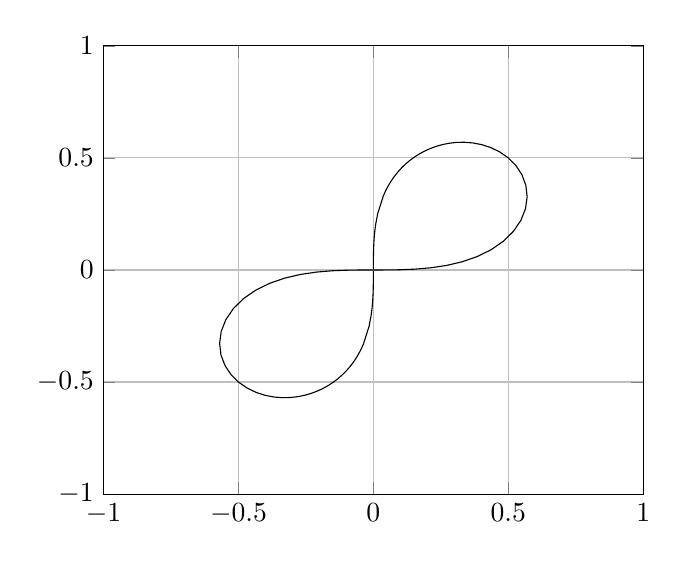
\begin{tikzpicture}
            \begin{axis}[
                xmin=-1,xmax=1,
                ymin=-1,ymax=1,
                grid=both,
                ]
                %TODO: Aumentar el tamaño para la versión final
                %Ponemos varios intervalos para minimizar las samples y, por tanto, el tiempo de compilación.
                \addplot [domain=-3:3,samples=100]({(x/(1+x^4))},{(x^3/(1+x^4))}); 
                \addplot [domain=-3:-50,samples=50]({(x/(1+x^4))},{(x^3/(1+x^4))}); 
                \addplot [domain=-50:-200,samples=50]({(x/(1+x^4))},{(x^3/(1+x^4))}); 
                \addplot [domain=3:50,samples=50]({(x/(1+x^4))},{(x^3/(1+x^4))}); 
                \addplot [domain=50:200,samples=50]({(x/(1+x^4))},{(x^3/(1+x^4))}); 
            \end{axis}
        \end{tikzpicture}
        \caption{\textit{Representación Lemniscata.}}
        \label{fig:lemniscata}
    \end{figure}

    Engañosamente: 
    \[
        \forall t \in \mathbb{R},\ \exists \left( t - \varepsilon, t + \varepsilon \right) = I_{\varepsilon}: f| : I_{\varepsilon} \rightarrow f\left( I_{\varepsilon} \right) 
    \]
    es homeomorfismo.

    En $t = 0, f\left( I_{\varepsilon} \right)$ \underline{no} es entorno de $f\left( 0 \right) = \left( 0, 0 \right)$, porque se tienen que tomar elementos de la rama ``vertical''.

    \item Las coordenadas polares $\left( 0, \rightarrow \right) \times \mathbb{R}^{} \rightarrow \mathbb{R}^{2},\ \left( r, \theta \right) \mapsto \left( r\cos \theta, r \sin \theta \right)$ es homeomorfismo local con $\theta_0 \in \left( \theta_0 - \pi, \theta_0 + \pi \right)$ hasta $\mathbb{R}^{2} \setminus L$ con $L$ la recta entre $O$ y $\theta_0$.
\end{enumerate} 
\end{ej}

\begin{defi}[Variedad Topológica]
Una \textbf{variedad topológica} de dimensión $m$ es un espacio localmente homeomorfo a $\mathbb{R}^m$, es decir, que cada punto tiene un entorno abierto homeomorfo a una bola\footnote{Luego, en el fondo, es homeomorfo a cualquier bola y, por ser éstas parte de una base de $\mathbb{R}^m$, es homeomorfo a todo $\mathbb{R}^m$.} $B\left( 0, \varepsilon \right) \subset \mathbb{R}^m$.
\end{defi}
\begin{ej}
Esferas, espacios proyectivos, toros...
\end{ej}

